\documentclass[aspectratio=169]{beamer}
\usepackage[utf8]{inputenc}
\usepackage[T1]{fontenc}
\usepackage[brazil]{babel}
\usepackage{ragged2e}
\usepackage{booktabs}
\usepackage{verbatim}
\usetheme{AnnArbor}
\usecolortheme{orchid}
\usefonttheme[onlymath]{serif}

\AtBeginSection[]{
  \begin{frame}
  \vfill
  \centering
  \begin{beamercolorbox}[sep=8pt,center,shadow=true,rounded=true]{title}
    \usebeamerfont{title}\insertsectionhead\par%
  \end{beamercolorbox}
  \vfill
  \end{frame}
}

%\title[\sc{Laboratório de Programação II -EC}]{Laboratório de Programação II -EC}
\title[\sc{Programação Orientada a Objetos - ECo}]{Programação Orientada a Objetos - ECo}
\author[Roland Teodorowitsch]{Roland Teodorowitsch}
%\institute[LP2 - EC - PUCRS]{Laboratório de Programação II - Curso de Engenharia de Computação - PUCRS}
\institute[POO - EC - PUCRS]{Programação Orientada a Objetos - ECo - Curso de Engenharia de Computação - PUCRS}
\date{1 de agosto de 2024}

\begin{document}
\justifying

%-------------------------------------------------------
\begin{frame}
	\titlepage
\end{frame}

%=======================================================
\section{Apresenta\c{c}\~ao da Disciplina}

%-------------------------------------------------------
\begin{frame}\frametitle{Sobre o professor}
\begin{itemize}
	\item Nome:
		\begin{itemize}
			\item Roland Teodorowitsch
		\end{itemize}
	\item Forma\c{c}\~ao:
		\begin{itemize}
			\item Bel. em Inform\'atica (PUCRS, 1990)
			\item Msc. em Ci\^encia da Computa\c{c}\~ao (UFRGS, 1994)
		\end{itemize}
	\item \'Areas de Interesse:
		\begin{itemize}
			\item SD, SO, STR, PP, Sist. Embarc., Arq. de Comp.
		\end{itemize}
	\item E-mail:
		\begin{itemize}
			\item roland.teodorowitsch@pucrs.br
		\end{itemize}
\end{itemize}
\end{frame}

%-------------------------------------------------------
\begin{frame}\frametitle{Sobre a disciplina}
\begin{itemize}
	%\item Nome: Laboratório de Programação II - EC
	%\item Código: 4610R
	\item Nome: Programação Orientada a Objetos - ECo
	\item Código: 98718-04
	\item Turma: 10
	\item Cr\'editos: 4
	\item Carga-horária: 60 horas-aula
	\item Hor\'ario:
	\begin{itemize}
		\item Turma 10: 2AB 4AB (AB=8h-9h30min)
		%\item Turma 11: 2CD 4CD (CD=9h45min-11h15min)
	\end{itemize}
	\item Modalidade: presencial
\end{itemize}
\end{frame}

%-------------------------------------------------------
\begin{frame}\frametitle{Sobre a disciplina}
\begin{itemize}
	\item Semestre: 2
	\item Pré-requisito:
		\begin{itemize}
			%\item Laboratório de Programação I -EC
			\item Introdução à Programação - ECo
		\end{itemize}
	\item Co-requisito:
		\begin{itemize}
			%\item Algoritmos e Estruturas de Dados II
			\item Algoritmos e Estruturas de Dados I
		\end{itemize}
	\item É pré-requisito para:
		\begin{itemize}
			%\item Sistemas Operacionais
			%\item Métodos Computacionais -EC
			\item Fundamentos do Processamento Paralelo e Distribuído
		\end{itemize}
\end{itemize}
\end{frame}

%-------------------------------------------------------
{%
\usebackgroundtemplate{
  \centering
  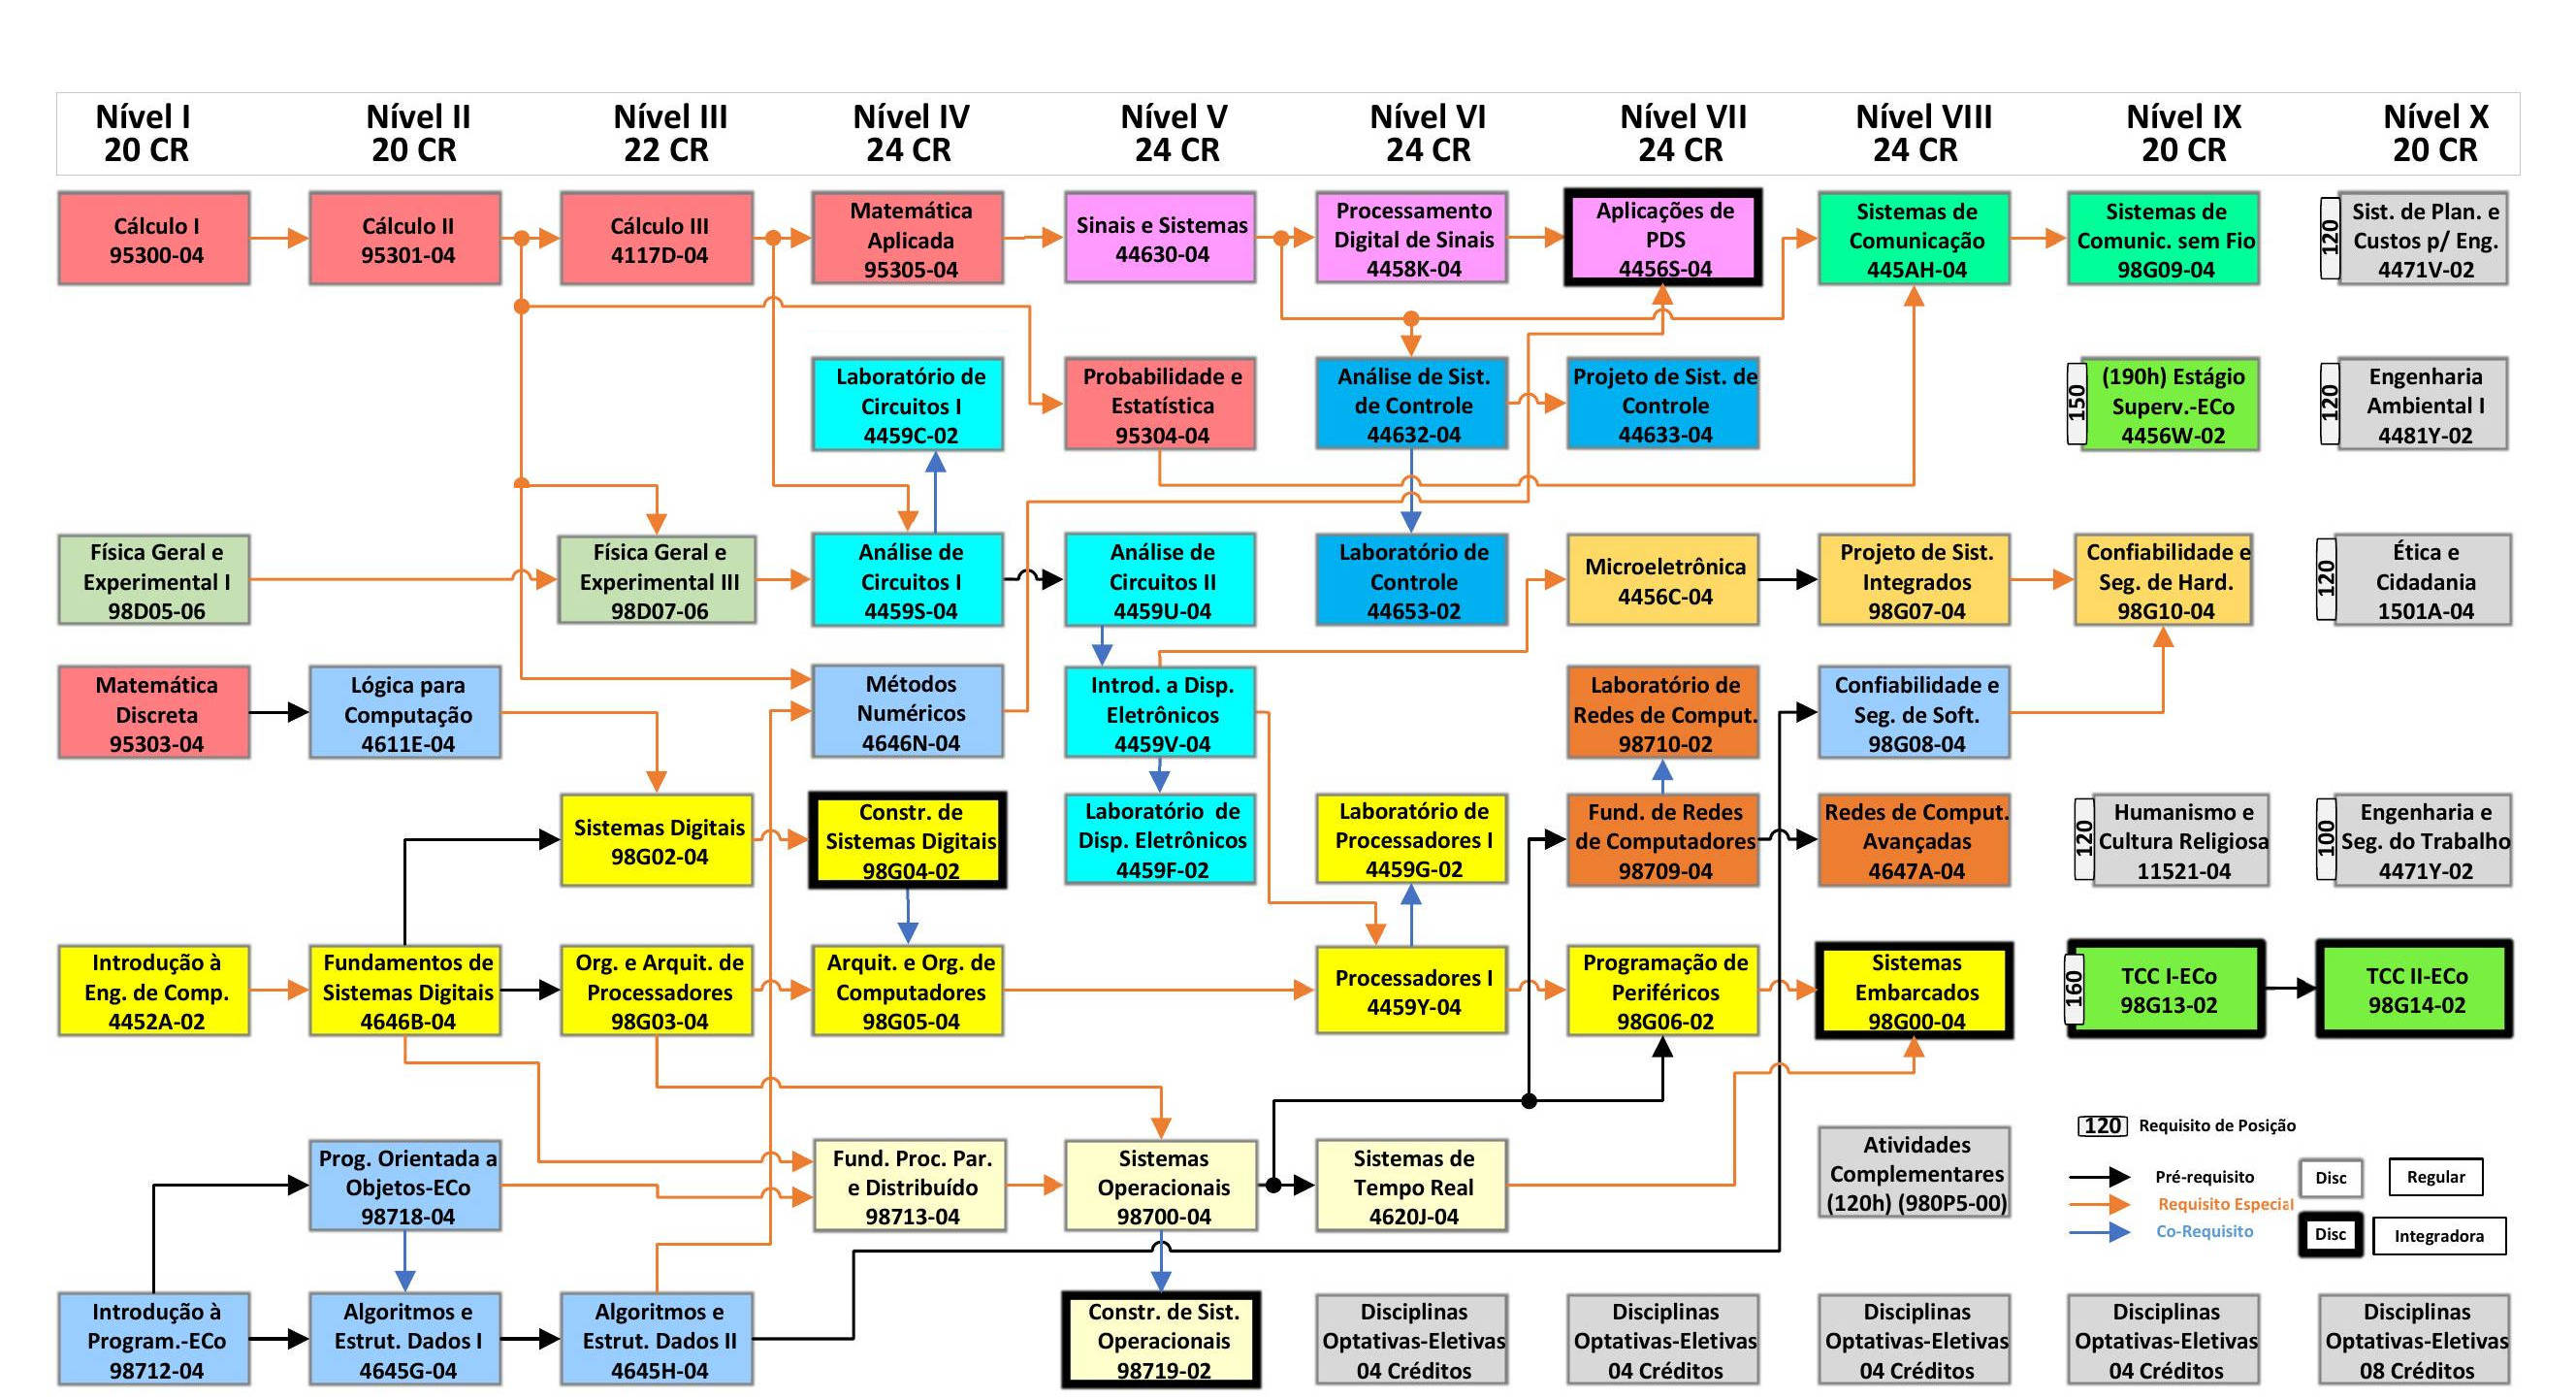
\includegraphics[width=\paperwidth]{pucrs-ec-poo-unidade_00-apresentacao_da_disciplina-laminas-matriz_curricular.jpg}
}
\begin{frame}\frametitle{}
\end{frame}
}

%-------------------------------------------------------
\begin{frame}\frametitle{Objetivos}
%O cumprimento da disciplina busca dar ao aluno, ao final do semestre, condições de:
%\begin{enumerate}
%	\item Compreender os conceitos fundamentais do paradigma de orientação de objetos;
%	\item Implementar ferramentas de \emph{software} utilizando uma linguagem orientada a objetos;
%	\item Continuar os estudos em programação avançada.
%\end{enumerate}
O cumprimento da disciplina busca dar ao aluno, ao final do semestre, condições de:
\begin{enumerate}
	\item Conhecer e utilizar de forma precisa conceitos e termos relacionados ao paradigma de orientação a objetos.
	\item Desenvolver as competências e habilidades para a criação de sistemas de complexidade média, formado por múltiplos componentes, e expressar estas soluções na forma de um sistema de classes em uma linguagem de programação.
	\item Empregar adequadamente ponteiros para manipulação de estruturas encadeadas e memória.
	\item Construir abstrações para tipos de dados, usando os conceitos de classe, objeto-mensagem, herança e polimorfismo.
	\item Compreender os conceitos avançados em orientação a objetos.
\end{enumerate}
\end{frame}

%=======================================================
\section{Conte\'udo}

%-------------------------------------------------------
\begin{frame}\frametitle{Ementa}
%Linguagem de programação imperativa e bloco-estruturada: subprogramas, recursividade, arquivos, tipos de dados estruturados, alocação dinâmica de memória. Estruturas avançadas, pré-processador, modularização. Programação orientada a eventos. Estilo de programação.
Paradigma de programação orientada a objetos; Abstração; Encapsulamento; Mensagens; Relacionamento entre classes (Composição, Referência); Parametrização de tipos (Templates); Uso de Ponteiros para Estruturas Encadeadas; Fluxos de Entrada e Saída; Modularização; Herança; Polimorfismo; STL; Conceitos avançados em Orientação a Objetos.
\end{frame}

%-------------------------------------------------------
\begin{frame}\frametitle{Conte\'udo (1/4)}
3 grandes unidades
\begin{itemize}
	\item Orientação a objetos básica
	\item Manipulação de dados
	\item Orientação a objetos avançada
\end{itemize}
\end{frame}

%-------------------------------------------------------
\begin{frame}\frametitle{Conte\'udo (2/4)}
\small{1. Orientação a objetos básica\\
~ 1.1. Conceitos de orientação a objetos\\
~ ~ 1.1.1. Classes e objetos\\
1.1.2. Atributos e métodos: classe e instância\\
~ 1.2. Visibilidade de atributos e métodos\\
~ 1.3. Princípios de projeto orientado a objetos\\
~ ~ 1.3.1. Mensagem\\
~ ~ 1.3.2. Abstração\\
~ ~ 1.3.3. Encapsulamento\\
~ 1.4. Detalhamento de classes\\
~ ~ 1.4.1. Relacionamento entre classes (composição, referência)\\
~ ~ 1.4.2. Construtores\\
~ ~ 1.4.3. Sobrecarga\\
~ ~ 1.4.4. Autorreferência\\
~ ~ 1.4.5. Modularização (agrupamento de classes relacionadas)}
\end{frame}

%-------------------------------------------------------
\begin{frame}\frametitle{Conte\'udo (3/4)}
2. Manipulação de dados\\
~ 2.1. Ponteiros\\
~ 2.2. Alocação dinâmica\\
~ 2.3. Estruturas encadeadas\\
~ 2.4. Fluxos de entrada e saída
\end{frame}

%-------------------------------------------------------
\begin{frame}\frametitle{Conte\'udo (4/4)}
3. Orientação a objetos avançada\\
~ 3.1. Generalização/especialização\\
~ ~ 3.1.1. Herança simples e múltipla\\
~ ~ 3.1.2. Hierarquia de classes\\
~ 3.2. Polimorfismo\\
~ 3.3. Tratamento de exceções\\
~ 3.4. Parametrização de tipos (\emph{Templates})\\
~ ~ 3.4.1. STL (\emph{Standard Template Library})\\
~ 3.5. Conceitos avançados em Orientação a Objetos
\end{frame}

%-------------------------------------------------------
\begin{frame}\frametitle{Bibliografia Básica}
%DEITEL, HARVEY M et al. \textbf{C++}: Como Programar. Porto Alegre : Bookman, 2001.\\
%~\\
%SCHILDT, H. \textbf{C++}: the complete reference. Berkeley: McGraw Hill, 1998.
RAMNATH, S.; DATHAN, B. \textbf{Object-Oriented Analysis, Design and Implementation}: an integrated approach. 2 ed. Heidelberg: Springer, 2010. 471 p. (ou anterior)\\
~\\
WEISFELD, M. \textbf{The Object-oriented Thought Process}. 4 ed. Upper Saddle River, NJ: Addison Wesley, 2013. 336 p.\\
~\\
MEYER, B. \textbf{Object Oriented Software Construction}. 2 ed. Upper Saddle River, NJ: Prentice Hall, 1997. 1296 p.
\end{frame}

%-------------------------------------------------------
\begin{frame}\frametitle{Bibliografia Complementar}
%JAMSA, K. \textbf{Aprendendo C++}. São Paulo: Makron Books, 1999.\\
%~\\
%SCHILDT, H. \textbf{Schildt's Expert C++}. Osborne MacGrawHill, 1996.\\
%~\\
%STROUSTRUP, B. \textbf{The C++ Programming Language}. Reading: Addison-Wesley, 1997.\\
%~\\
%ZEIGLER, B. \textbf{Objects and systems}: principled design with implementations in C++ and Java. Springer, 1997.
BOOCH, G. et al. \textbf{Object-oriented Analysis and Design with Applications}. 3rd ed. Upper Saddle River, NJ: Addison Wesley, 2007. 720 p. (ou anterior)\\
%~\\
DEITEL, H. M; DEITEL, P. J. \textbf{C++}: como programar. 5 ed. São Paulo: Pearson Education do Brasil, 2006. 1208 p. (ou anterior)\\
%~\\
FARRELL, J. \textbf{An Object-oriented Approach to Programming Logic and Design}. 4 ed. Boston, MA: Cengage Learning, 2012. 560 p.\\
%~\\
GAMMA, E. et al. \textbf{Padrões de Projeto}: soluções reutilizáveis de software orientado a objetos. Porto Alegre: Bookman, 2000. 364 p.\\
%~\\
SILVA Fo., A. M. \textbf{Introdução a Programação Orientada a Objetos com C++}. Rio de Janeiro, RJ: Elsevier/Campus, 2010. 312 p.
\end{frame}

%=======================================================
\section{Avalia\c{c}\~ao}

%-------------------------------------------------------
\begin{frame}\frametitle{Avalia\c{c}\~ao}
\[
G1 = \frac{ 2 \times MT + 4 \times P_1 + 4 \times P_2}{10}
\]
\begin{itemize}
%	\item $E$ = Média das listas de exercícios ($E_1$ a $E_7$)
%	\item $T1$ = Trabalho 1
%	\item $T2$ = Trabalho 2
	\item $MT$ = Média de Trabalhos
 	\item $P_1$ = Prova referente à primeira parte da disciplina
	\item $P_2$ = Prova referente a todo o conteúdo da disciplina
\end{itemize}
\end{frame}

\begin{comment}
%-------------------------------------------------------
\begin{frame}\frametitle{Avalia\c{c}\~ao (até 2019/2)}
\[
G1 = \frac{P_1 + P_2 + M_{trab}}{3}
\]
\begin{itemize}
	\item $P_1$ = prova referente \`as unidades 1 e 2
	\item $P_2$ = prova referente \`as unidades 2 e 3
	\item $T$ = média dos trabalhos práticos
\end{itemize}
\end{frame}

%-------------------------------------------------------
\begin{frame}\frametitle{Avalia\c{c}\~ao (Remoto)}
\[
G1 = 0,25 \times T_1 + 0,30 \times T_2 + 0,25 \times ME + 0,2 \times AA
\]
\begin{itemize}
	\item $T_1$ = trabalho prático 1
	\item $T_2$ = trabalho prático 2
	\item $ME$ = média de exercícios desenvolvidos ao longo do semestre
	\item $AA$ = atividade avaliativa \emph{on-line} assíncrona (ou prova final)
\end{itemize}
\end{frame}
%-------------------------------------------------------
\begin{frame}\frametitle{Avalia\c{c}\~ao}
\[
G1 = \frac{P_1 + P_2 + T}{3}
\]
\begin{itemize}
	\item $P_1$ = prova referente \`as unidades 1, 2 e 3
        \item $P_2$ = prova referente \`as unidades 4, 5, 6 e 7
	\item $T$ = média dos trabalhos práticos
\end{itemize}
\end{frame}
\end{comment}

%-------------------------------------------------------
\begin{comment}
\begin{frame}\frametitle{Trabalhos}
	\begin{itemize}
		\item $T_1$ = Trabalho de implementação
		\begin{itemize}
			\item 2013/2: Razão Monotônica (RM)
			\item 2014/1: \emph{Deadline} Monotônico (DM)
			\item 2014/2: \emph{Earliest Deadline First} (EDF)
			\item 2015/1: \emph{Background Server} (BS)
			\item 2015/2: Razão Monotônica (RM)
			\item 2016/1: \emph{Least Slack Time first} (LST)
			\item 2016/2: \emph{Polling Server} (PS)
			\item 2017/1: \emph{Deadlines} Arbitrários
			\item 2017/2: POSIX 1003b
			\item 2018/1: ???
		\end{itemize}
		\item $T_2$ = Seminário
	\end{itemize}
\end{frame}
\end{comment}

%-------------------------------------------------------
\begin{frame}\frametitle{\'Indices de Aprova\c{c}\~ao}
	\begin{table}
		\centering
		\small
		\begin{tabular}{cccccccc}
			\toprule
			SEM. & N\'UM. AL. & APROV. & REP. & REP. FALTAS & CANC. & CANC. NC\\
			\midrule
			2019/1 & 14 & 10 (71,4\%) & 1 (7,1\%) & 1 (7,1\%) & 2 (14,3\%)& 0 (0,0\%)\\
			2019/2 & 25 & 16 (64,0\%) & 2 (8,0\%) & 0 (0,0\%) & 7 (28,0\%)& 0 (0,0\%)\\
			2020/1 & 13 & 2 (15,4\%) & 3 (23,1\%) & 0 (0,0\%) & 8 (61,5\%)& 0 (0,0\%)\\
			2020/2 & 31 & 17 (54,8\%) & 4 (12,9\%) & 0 (0,0\%) & 10 (32,3\%)& 0 (0,0\%)\\
			2021/1 & 17 & 6 (35,3\%) & 2 (11,8\%) & 0 (0,0\%) & 9 (52,9\%)& 0 (0,0\%)\\
			2021/2 & 27 & 9 (33,3\%) & 11 (40,7\%) & 0 (0,0\%) & 2 (7,4\%)& 5 (18,5\%)\\
			2022/1 & 31 & 10 (32,3\%) & 4 (12,9\%) & 2 (6,5\%) & 12 (38,7\%)& 3 (9,7\%)\\
			2022/2 & 12 & 3 (25,0\%) & 1 (8,3\%) & 1 (8,3\%) & 7 (58,3\%)& 0 (0,0\%)\\
			2023/1 & 20 & 11 (55,0\%) & 2 (10,0\%) & 3 (15,0\%) & 4 (20,0\%)& 0 (0,0\%)\\
			2023/2 (10) & 9 & 4 (44,4\%) & 2 (22,2\%) & 0 (0,0\%) & 3 (33,3\%) & 0 (0,0\%)\\
			2023/2 (11) & 23 & 13 (56,5\%) & 2 (8,7\%) & 1 (4,3\%) & 7 (30,4\%) & 0 (0,0\%)\\
			2024/1 & 21 & 8 (38,1\%) & 2 (9,5\%) & 3 (14,3\%) & 7 (33,3\%) & 1 (4,8\%)\\
			\bottomrule
		\end{tabular}
		\caption{\'Indices de Aprova\c{c}\~ao}
	\end{table}
\end{frame}

%=======================================================
\section{Informa\c{c}\~oes Gerais}

%-------------------------------------------------------
\begin{frame}\frametitle{Avisos: Presenças e Faltas}
\begin{itemize}
	\item 1 encontro = 2 presen\c{c}as ou faltas
	\item em 2024-2: 34 encontros (68 horas/aula) com presença contabilizada
	\item na semana de G2, a presença NÃO é contabilizada
	\item frequ\^encia m\'inima para aprova\c{c}\~ao: 75\%
	\item limite de faltas = 25\% de 68 = 17
	\item portanto, com 17 faltas (8 encontros e meio) o aluno está REPROVADO POR FALTAS
\end{itemize}
\end{frame}

%-------------------------------------------------------
\begin{frame}\frametitle{Avisos: Moodle}
\begin{itemize}	
	\item Avisos pelo Mural
	\item D\'uvidas pelo f\'orum
	\item Material de apoio
	\item Entrega de trabalhos e exerc\'icios
\end{itemize}
\end{frame}

%-------------------------------------------------------
\begin{frame}\frametitle{Avisos: Diversos}
\begin{itemize}
	\item Listas de exercícios com múltiplas entregas
%	\item Avaliação personalizada
\end{itemize}
\end{frame}

%-------------------------------------------------------
\begin{frame}\frametitle{Avisos: Mapas Mentais}
\begin{itemize}
	\item São uma forma de representar conhecimento sobre determinado assunto
	\item Recomenda-se fortemente que o aluno construa Mapas Mentais dos conteúdos da disciplina
	\item Os Mapas Mentais poderão ser usados nas avaliações da disciplina (com exceção das provas PS e G2)
	\item Regras:
	\begin{itemize}
		\item Um Mapa Mental por unidade do conteúdo programático
		\item NÃO incluir textos grandes e/ou copiados e colados nos nodos do mapa
		\item Cada Mapa Mental em uma folha A4 impressa
		\item Todos os Mapas Mentais devem ser entregues uma semana antes da avaliação em que serão utilizados
	\end{itemize}
	\item Mapas Conceituais também são uma alternativa interessante
\end{itemize}
\end{frame}

%-------------------------------------------------------
\begin{frame}\frametitle{Avisos: Recomendações}
\begin{itemize}
	%\item Realizar as leituras indicadas antes da aula
	\item Dificuldades não esclarecidas em disciplinas anteriores NÃO serão resolvidas sem esforço adicional
	\item Consultem as obras disponíveis na biblioteca (livros físicos e on-line)
	\item Aproveitar a aula para realizar os exercícios
	\item Não deixe acumular trabalhos
	\item Não se aprende a programar estudando na véspera da prova...
	\item Reserve um horário de estudo na semana para cada uma das disciplinas
	\item "Disciplina é liberdade..." (letra da música Há Tempos, da banda Legião Urbana)
	\item Existe uma monitoria que presta apoio aos alunos com dúvidas (verifique horários na página de monitoria)
\end{itemize}
\end{frame}

\begin{comment}
%-------------------------------------------------------
\begin{frame}\frametitle{Avisos: Diversos}
\begin{itemize}
    \item Em todos os horários da disciplina, o professor estará \emph{on-line} no Zoom
    \item Na maioria dos tópicos, haverá uma aula expositiva (via Zoom ou via vídeo disponibilizado no YouTube) seguida de uma aula de exercícios para entrega
    \item No moodle, há um \emph{link} com convite para o grupo de Whatsapp
%	\item Método 300
%	\item Presenças e faltas devem ser acompanhadas pelo aplicativo
%	\item Avaliação personalizada
\end{itemize}
\end{frame}
\end{comment}

%=======================================================
\section{Dúvidas?}

%-------------------------------------------------------
\begin{frame}\frametitle{Dúvidas?}
	\begin{figure}[h]
		\centering
		
\includegraphics[height=0.6\paperheight]{pucrs-ec-poo-unidade_00-apresentacao_da_disciplina-laminas-duvidas.png}
	\end{figure}
\end{frame}

%=======================================================
\section{Mensagens Finais}

\begin{comment}
%-------------------------------------------------------
\begin{frame}\frametitle{Mensagens Finais}
	\begin{figure}[h]
		\centering
		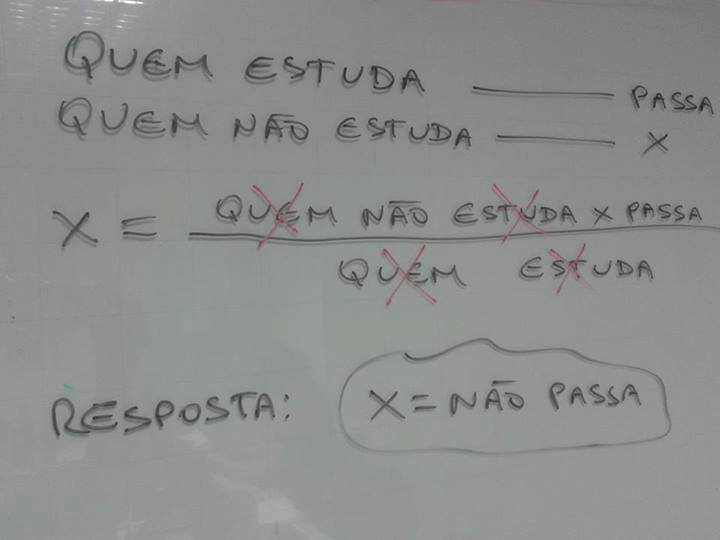
\includegraphics[height=0.6\paperheight]{pucrs-ec-poo-unidade_00-apresentacao_da_disciplina-laminas-quem_estuda.jpg}
		\caption{https://www.facebook.com/acreditesouengenheiro}\label{quemEstuda}
	\end{figure}
\end{frame}
\end{comment}

%-------------------------------------------------------
\begin{frame}\frametitle{Reflexões}
\url{https://youtu.be/eBGRY6aeaqA}
\end{frame}

\begin{comment}	
%-------------------------------------------------------
\begin{frame}\frametitle{Reflexões}
	\begin{block}{Plat\~ao}
		O objetivo da educação é o de nos ensinar a amar a beleza.
	\end{block}
	\begin{block}{Aristóteles}
		A educação tem raízes amargas, mas os seus frutos são doces.\\
		~\\
		É fazendo que se aprende a fazer aquilo que se deve aprender a fazer.\\
		~\\
		A alegria que se tem em pensar e aprender faz-nos pensar e aprender ainda mais.\\
		~\\
		A primeira qualidade do estilo é a clareza.
	\end{block}
\end{frame}

%-------------------------------------------------------
\begin{frame}\frametitle{Reflexões}
	\begin{block}{Albert Einstein}
		A única coisa que interfere com meu aprendizado é a minha educação.
	\end{block}
	\begin{block}{Epicteto}
		É impossível para um homem aprender aquilo que ele acha que já sabe.
	\end{block}
	\begin{block}{Ralph Waldo Emerson}
		O que é ensinado em escolas e universidades não representa educação, mas são meios para obtê-la.
	\end{block}
	\begin{block}{Derek Bok}
		Se você acha que educação é cara, experimente a ignorância.
	\end{block}
\end{frame}

%-------------------------------------------------------
\begin{frame}\frametitle{Reflexões}
	\begin{block}{Confúcio}
		Quem, revendo o antigo, aprende o novo, pode ser considerado mestre.
	\end{block}
	\begin{block}{Benjamin Franklin}
		Conte me algo e eu esquecerei. Mostre-me algo e talvez eu lembre. Envolva-me e eu aprenderei.
	\end{block}
	\begin{block}{Albert Einstein}
		Quem nunca errou nunca experimentou nada novo.
	\end{block}
	\begin{block}{Albert Einstein}
		Nunca deixe o medo de errar impedir que você jogue.
	\end{block}

\end{frame}

%-------------------------------------------------------
\begin{frame}\frametitle{Reflexões}
	\begin{block}{Cora Coralina}
		Feliz aquele que transfere o que sabe e aprende o que ensina.
	\end{block}
	\begin{block}{Guimarães Rosa}
		Mestre não é quem sempre ensina, mas quem de repente aprende.
	\end{block}
	\begin{block}{Georges Duhamel}
		O bom mestre aprende com as lições que dá.
	\end{block}
\end{frame}

%-------------------------------------------------------
\begin{frame}\frametitle{Reflexões}
	\begin{block}{Mahatma Gandhi}
		Viva como se fosse morrer amanhã. Aprenda como se fosse viver para sempre.
	\end{block}
	\begin{block}{Albert Einstein}
		Nunca pare de aprender, porque a vida nunca para de ensinar.
	\end{block}
	\begin{block}{Albert Einstein}
		Quando você para de aprender, você começa a morrer.
	\end{block}
\end{frame}
\end{comment}

%-------------------------------------------------------
\begin{frame}\frametitle{Bem-vindos}
	\begin{figure}[h]
		\centering
		
\includegraphics[height=0.7\paperheight]{pucrs-ec-poo-unidade_00-apresentacao_da_disciplina-laminas-welcome.jpg}
	\end{figure}
\end{frame}

%-------------------------------------------------------
\end{document}

